\documentclass[12pt,a4paper]{article}
\usepackage[UTF8]{ctex}
\usepackage{graphicx}
\usepackage{geometry}
\usepackage{ulem}
\usepackage{enumitem}
\usepackage{titlesec}
\usepackage{multicol}
\usepackage[export]{adjustbox}
\usepackage{amsmath}  % 推荐用于更好的数学排版
\usepackage[utf8]{inputenc}
\usepackage{CJKutf8}
\usepackage{fancyhdr}
\usepackage{lastpage}
\usepackage{ulem}
\usepackage{tabularx}
\usepackage{lastpage}
\usepackage{float}
% 页眉页脚设置
\pagestyle{fancy}
\fancyhf{} % 清除所有页眉页脚
% 设置页眉内容
%-==========1. 填写从第二页开始 每页第一行的信息==========-
\fancyhead[C]{
    \makebox[4.5em][c]{实验名称：} \uline{\makebox[14em][c]{一阶RC电路瞬态响应过程实验}} 
    \makebox[2.5em][c]{姓名：} \uline{\makebox[4em][c]{}} 
    \makebox[2.5em][c]{学号：} \uline{\makebox[5em][c]{}}
}%--------------------------------------------------------
\fancyfoot[C]{第 \thepage\ 页，共 \pageref{LastPage} 页}

% 取消页眉和页脚的下划线
\renewcommand{\headrulewidth}{0pt} % 页眉横线粗细设为0
\renewcommand{\footrulewidth}{0pt} % 页脚横线粗细设为0

% 调整页眉高度
\setlength{\headheight}{50pt}

% 设置plain样式（用于第一页）
\fancypagestyle{plain}{
    \fancyhf{} % 清除所有页眉页脚
    \renewcommand{\headrulewidth}{0pt} % 隐藏页眉横线
    \fancyfoot[C]{第 \thepage\ 页，共 \pageref{LastPage} 页} % 保留页脚
}
% 设置页面边距
\geometry{left=2.54cm,right=1.5cm,top=2.54cm,bottom=2.54cm}

% 设置正文字体大小为小四
\renewcommand{\normalsize}{\fontsize{12pt}{18pt}\selectfont}
% 设置章节格式
\titleformat{\section}{\fontsize{16pt}{24pt}\selectfont\bfseries}{\thesection}{1em}{} % 一级标题：三号
\titleformat{\subsection}{\fontsize{15pt}{22.5pt}\selectfont\bfseries}{\thesubsection}{1em}{} % 二级标题：小三

\begin{document}
\thispagestyle{plain}%第一页使用 plain 样式，而不是默认的 fancy 样式，第一页不再显示页眉
% 标题部分 - 两栏布局
\begin{multicols}{2}
    % 左栏：图片和实验报告标题
    % 左栏：使用空行创建前三行
    \noindent
    ~\\ % 第一行
    ~\\ % 第二行
    ~\\ % 第三行
    \hphantom{占位}% 使用空占位符
    \raisebox{-0.5\baselineskip}% 图片向下移动半行
    {
\includegraphics[width=1.85in,height=0.58in]{figure/ZJU.jpg}}
    \hspace{.5em}% 图片和标题之间的间距
    \raisebox{0pt}[\height][0pt]% 标题底部对齐
    {\textbf{\fontsize{26pt}{30pt}\selectfont 实验报告}}
    
    \columnbreak % 换到右栏
    
    % 右栏：个人信息
    % 右栏：个人信息 - 靠右对齐 
%-==========2. 填写个人信息==========-
    \begin{flushright}
        \makebox[3em][l]{专业：} \uline{\makebox[9em][c]{}} \\
        \makebox[3em][l]{姓名：} \uline{\makebox[9em][c]{}} \\
        \makebox[3em][l]{学号：} \uline{\makebox[9em][c]{}} \\
        \makebox[3em][l]{日期：} \uline{\makebox[9em][c]{2025年11月18日}} \\
        \makebox[3em][l]{地点：} \uline{\makebox[9em][c]{紫金港东四216}} \\
    \end{flushright}   
\end{multicols}
% 课程名称等信息（单栏）
%-==========3. 填写课程信息==========-
\noindent\small
课程名称： \uline{电子电路设计实验I} \hfill 指导老师： \uline{施红军、叶险峰、邓靖靖} \hfill 成绩： \uline{\hspace{3cm}} \\
实验名称： \uline{一阶RC电路瞬态响应过程实验} \hfill 实验类型： \uline{探究类} \hfill 同组学生姓名： \uline{}
%-==========4. 正文开始==========-
\section*{一、实验目的}
1.掌握示波器的使用方法，学会利用示波器稳定波形，使用自动测量法和光标法测量波形的周期、幅值等参数。

2.了解RC电路的零输入响应和零状态响应，掌握测量RC电路时间常数的方法。

\section*{二、实验任务与要求}
1.观察输入的方波信号波形，测量其周期。

2.理论计算RC电路的时间常数，并通过实验测量RC电路的时间常数，比较计算值与测量值。

\section*{三、实验原理}
1.一阶RC电路的零状态响应

\begin{figure}[H]
    \centering
    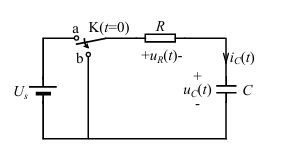
\includegraphics[width=0.4\textwidth, height=0.2\textheight]{figure/RC_circuit.png}
    \caption{一阶电路}
    \label{fig:3.1}
\end{figure}

如图\ref{fig:3.1}所示，对于一阶RC电路，开关置于a点，当初始电压为零时，电路的响应称为零状态响应。设输入信号为阶跃信号$u_s(t)$，则电容器上的电压$u_c(t)$满足以下微分方程：
\begin{equation}
    RC \frac{du_c(t)}{dt} + u_c(t) = u_s(t)
\end{equation}
解该微分方程可得零状态响应为：
\begin{equation}
    u_c(t) = u_s(1 - e^{-\frac{t}{RC}})
\end{equation}
其中，$RC$为时间常数，表示电路响应的快慢。

2.一阶RC电路的零输入响应
当开关置于b点时，电路的响应称为零输入响应。设初始电压为$U_0$，则电容器上的电压$u_c(t)$满足以下微分方程：
\begin{equation}
    RC \frac{du_c(t)}{dt} + u_c(t) = 0
\end{equation}
解该微分方程可得零输入响应为：
\begin{equation}
    u_c(t) = U_0 e^{-\frac{t}{RC}}
\end{equation}
其中，$RC$为时间常数，表示电路响应的快慢。

3.方波响应

方波信号是一种周期性变化的信号，具有固定的高电平和低电平时间。对于一阶RC电路，当输入为方波信号时，电路会经历充电和放电过程，分别对应零状态响应和零输入响应。
当方波周期足够长时就可以根据占空比选择合适的时间段来观察零状态响应和零输入响应，从而测量时间常数。

占空比高的方波对应的响应可以视为零状态响应，而占空比低的方波对应的响应可以视为零输入响应。

由此可以实现重复激励电路，得到期望响应。
\section*{四、实验方案设计与参数计算}
\subsection*{4.1 实验方案总体设计}

\begin{figure}[H]
    \centering
    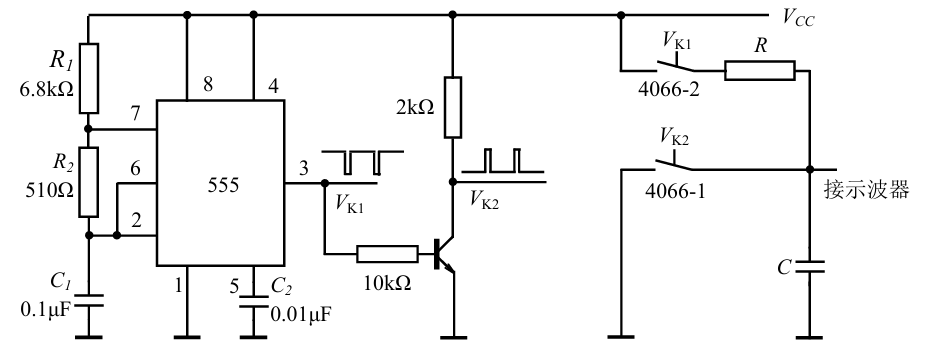
\includegraphics[width=0.4\textwidth, height=0.2\textheight]{figure/circut_design.png}
    \caption{重复激励的零状态响应观测实验电路图}
    \label{fig:4.1}
\end{figure}

\begin{figure}[H]
    \centering
    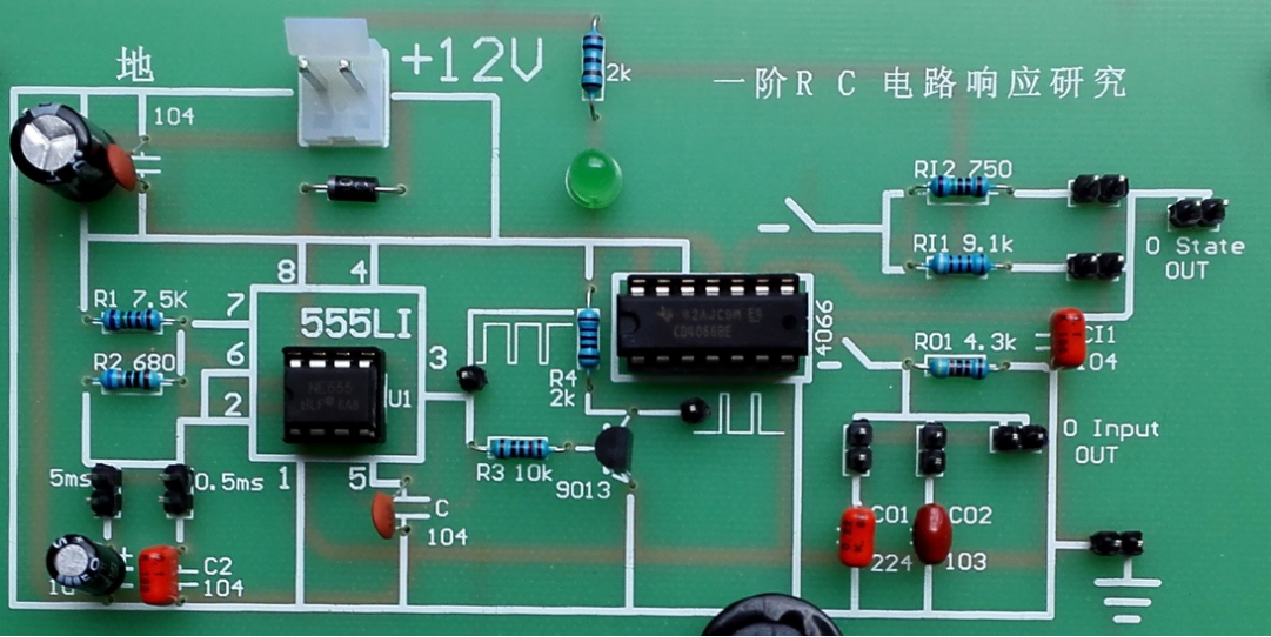
\includegraphics[width=0.4\textwidth, height=0.2\textheight]{figure/real_circuit.png}
    \caption{电路实物}
    \label{fig:4.1.2}
\end{figure}
 RC 电路的响应是一个十分短暂的单次变化瞬态过程，一次激励引起电路一次响应。要在示波
器上显示RC电路的响应曲线进而进行观察和测量有关参数，就必须周期性地重复进行激励，使这
种单次变化的过程重复出现，而且要保证激励信号与示波器扫描的同步，只有这样，才能在示波器
上显示稳定的电路响应曲线。 

为此，实验时必须设计一个实验方案，实现对RC电路的周期性重复激励和向示波器提供扫描
同步信号。图\ref{fig:4.1} 是观测零状态响应过程的实验电路，选用 555 时基电路作激励脉冲信号发生电
路，用CD4066电子开关实现电路中开关的切换，脉冲信号的前沿为示波器提供扫描同步触发信号。

电路实物组装图如\ref{fig:4.1.2}所示。
\subsection*{4.2 各功能电路设计与计算}
实验涉及到四组RC电路，需要分别计算并测量时间常数。

计算结果如下表所示：
\begin{table}[H]
\footnotesize
\caption{\normalsize RC电路参数计算值} 
\centering  
\renewcommand{\arraystretch}{1.1}
\begin{tabular}{*{4}{l}} 
\hline\hline   
$R(\Omega)$ &$C(pF)$ &$\tau$ 计算值(ms) &$5 \tau$ 计算值(ms) \\ 
\hline
9.1K & $1 \times 10^{5}$& 0.910& 4.550\\
750 & $1 \times 10^{5}$& 0.075& 0.375\\
4.3K & $1 \times 10^4$& 0.043& 0.215\\
4.3K & $2.2 \times 10^5$& 0.946& 4.730\\
\hline  
    \end{tabular}
    \label{table:4.2}
\end{table}

\section*{五、实验仪器设备}
电路板，示波器，恒压源等。

\section*{六、实验步骤、调试过程、实验数据记录}
\subsection*{1.观察方波响应}
实验使用方波作为RC电路的激励信号，方波由信号发送电路产生，具有5ms和0.5ms两种类型。
实验通过示波器分别观察两种激励信号的波形，并测量周期。

\begin{table}[H]
\footnotesize
\caption{\normalsize  方波激励信号周期测量结果} 
\centering  
\renewcommand{\arraystretch}{1.1}
\begin{tabular}{*{3}{l}} 
\hline\hline   
理论周期 &测量周期 &波形  \\ 
\hline
5ms & 5.5800ms& 见图\ref{fig:6.1} \\
0.5ms & 0.58060ms& 见图\ref{fig:6.2} \\
\hline  
    \end{tabular}
    \label{table:6.1.1}
\end{table}

\begin{figure}[H]
    \centering
    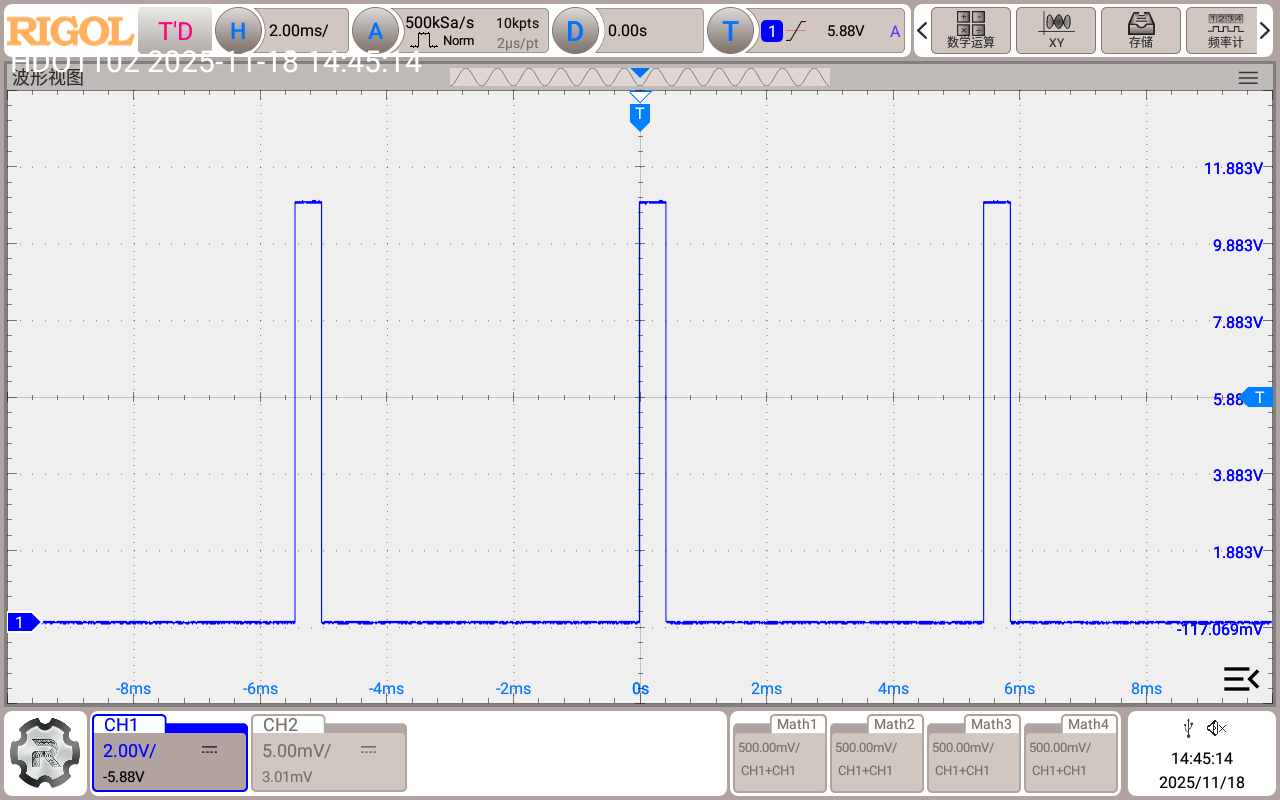
\includegraphics[width=0.4\textwidth, height=0.2\textheight]{figure/c5input0.png}
    \caption{5ms方波波形图}
    \label{fig:6.1}
\end{figure}

\begin{figure}[H]
    \centering
    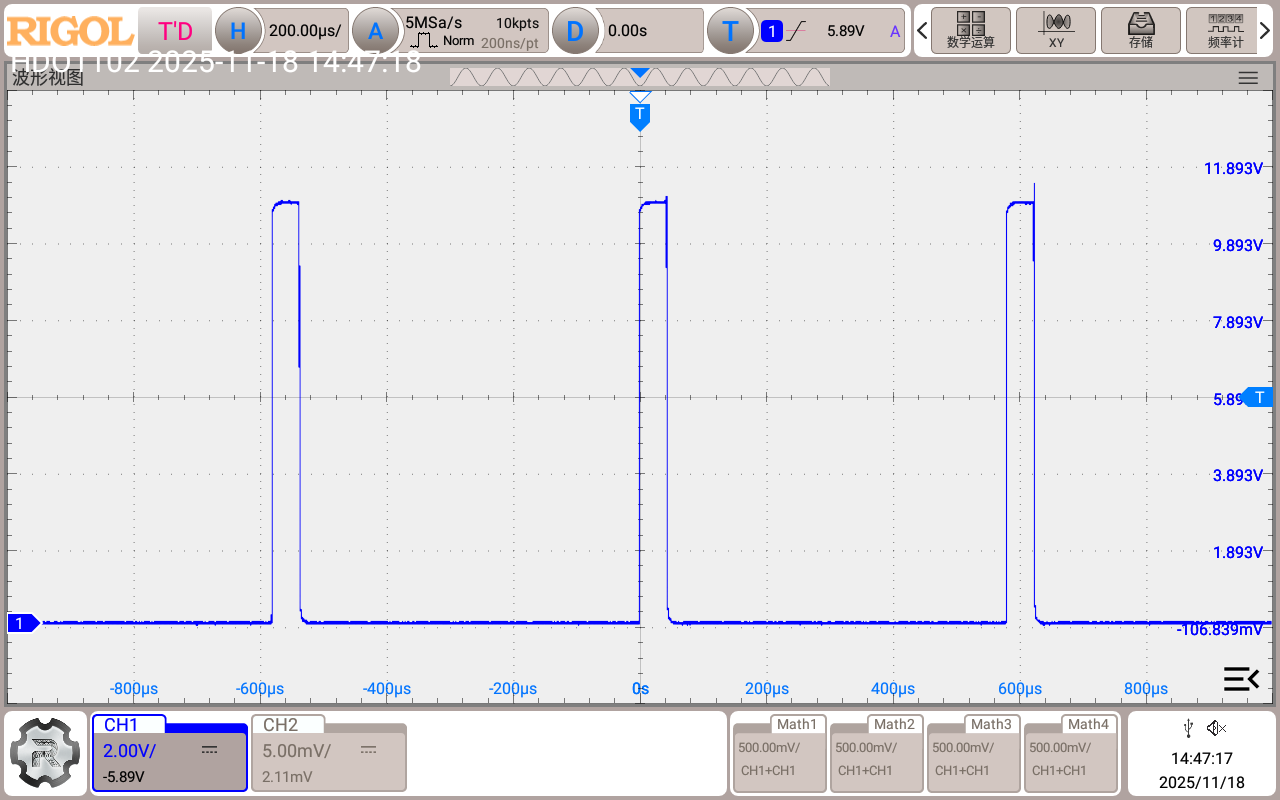
\includegraphics[width=0.4\textwidth, height=0.2\textheight]{figure/c0.5input0.png}
    \caption{0.5ms方波波形图}
    \label{fig:6.2}
\end{figure}

\subsection*{2.测量RC电路的零状态响应时间常数}
实验过程中通过改变电阻来改变时间常数，选择不同周期的方波作为激励，记录响应波形，并测量时间常数。
时间常数测量方法是首先在测量波形最大值$u_s$并波形上任取一点$u_c(t_0)$，计算出$u_c(t_0+ \tau)=0.632(u_s - u_c(t_0)) + u_c(t_0)$。
通过示波器测量出$t_0 + \tau$对应的时间点，从而计算出时间常数$\tau$。

实验测量结果如下表所示：
\begin{table}[H]
\footnotesize
\caption{\normalsize  RC电路零状态响应时间常数测量结果} 
\centering  
\renewcommand{\arraystretch}{1.1}
\begin{tabular}{*{7}{l}} 
\hline\hline   
$R(\Omega)$ &$C(pF)$ &波形&$\tau$ 测量值(ms) &$u_c(t_0)(V)$ &$u_c(t_0 + \tau)(V)$ &$u_s(V)$\\ 
\hline
9.1K & $1 \times 10^{5}$& 见图\ref{fig:6.3} & 0.980& 1.915&7.794&11.218\\
750 & $1 \times 10^{5}$& 见图\ref{fig:6.4} & 0.086& 2.293 & 8.039 & 11.385\\
\hline  
    \end{tabular}
    \label{table:6.1}
\end{table}

\begin{figure}[H]
    \centering
    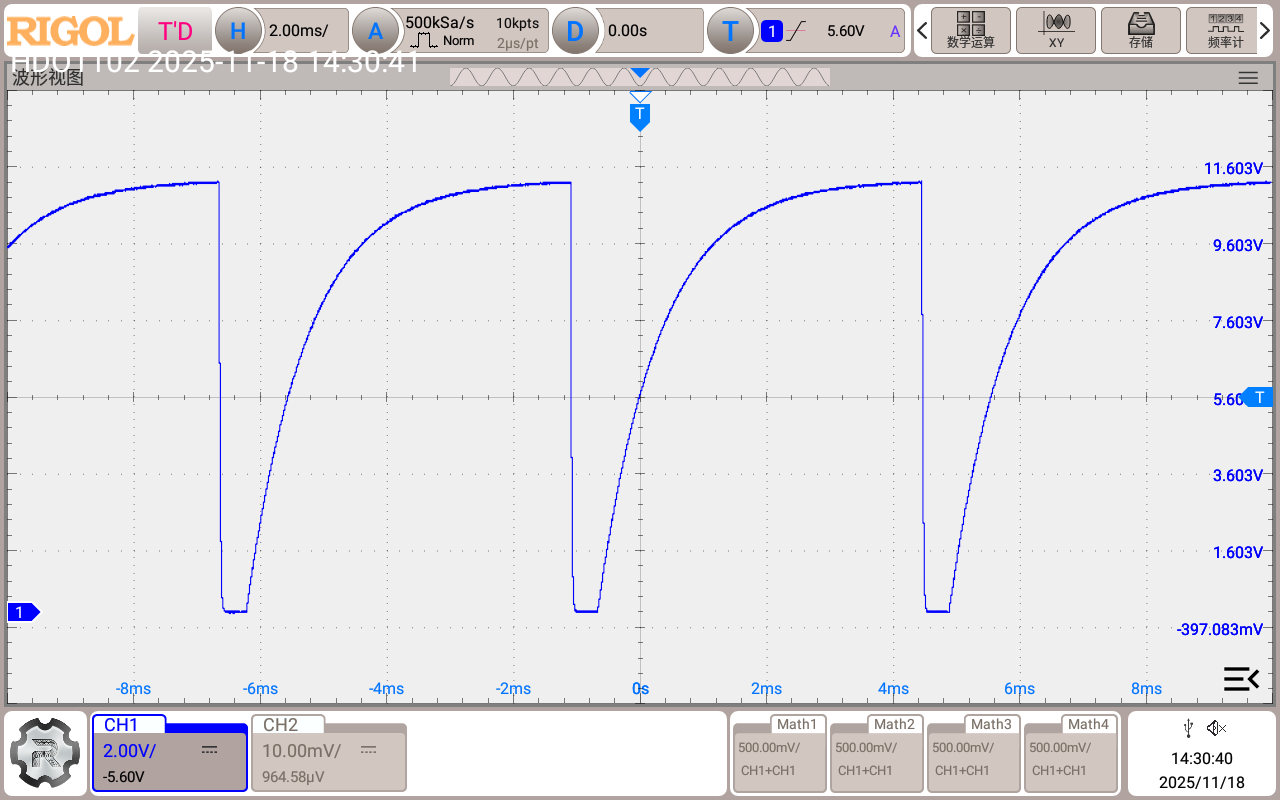
\includegraphics[width=0.4\textwidth, height=0.2\textheight]{figure/c91001050.png}
    \caption{$R=9.1k \Omega, C=1 \times 10^{5} pF$零状态响应波形图}
    \label{fig:6.3}
\end{figure}
\begin{figure}[H]
    \centering
    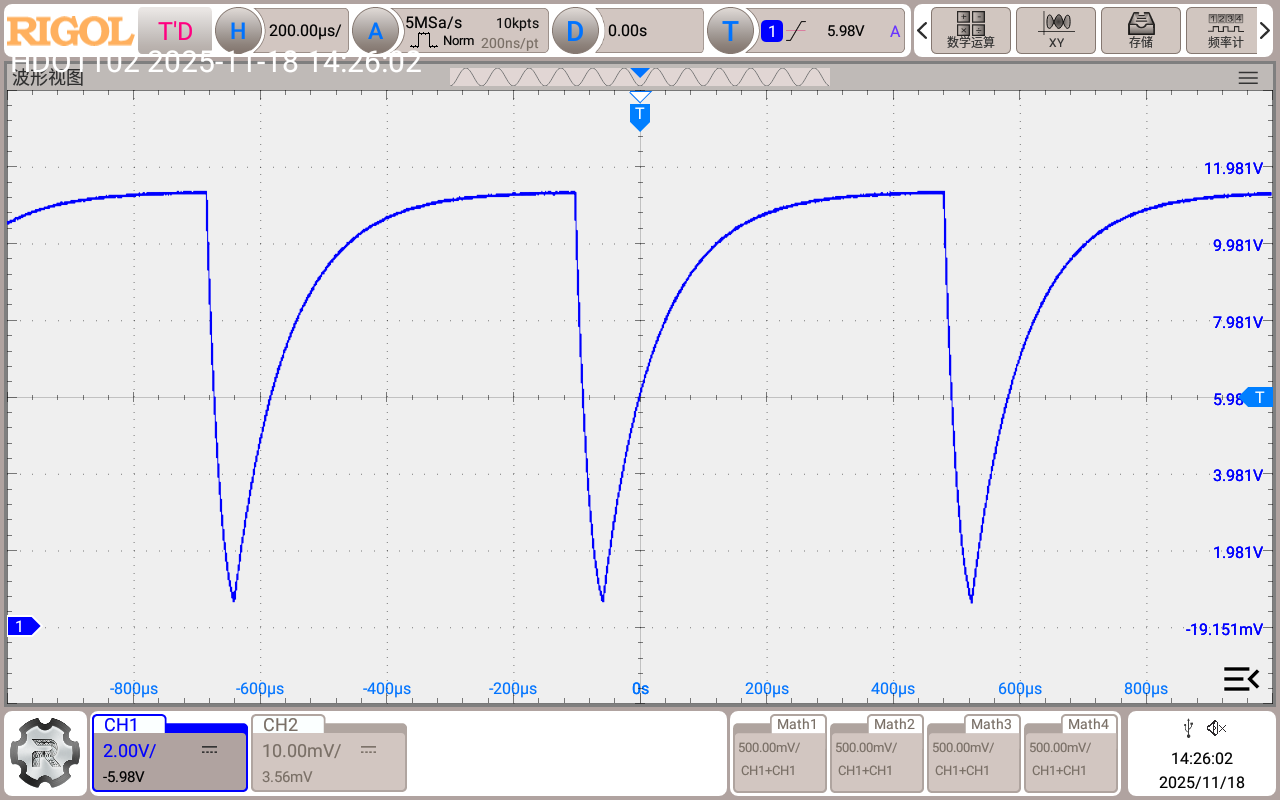
\includegraphics[width=0.4\textwidth, height=0.2\textheight]{figure/c7501050.png}
    \caption{$R=750 \Omega, C=1 \times 10^{5} pF$零状态响应波形图}
    \label{fig:6.4}
\end{figure}
\subsection*{3.测量RC电路的零输入响应时间常数}
实验通过改变电容来改变时间常数，选择不同周期的方波作为激励，记录响应波形，并测量时间常数。
时间常数测量方法是首先在波形上任取一点$u_c(t_0)$，计算出$u_c(t_0+ \tau)=u_c(t_0) \times 0.368$。
通过示波器测量出$t_0 + \tau$对应的时间点，从而计算出时间常数$\tau$。
实验测量结果如下表所示：
\begin{table}[H]
\footnotesize
\caption{\normalsize  RC电路零输入响应时间常数测量结果} 
\centering  
\renewcommand{\arraystretch}{1.1}
\begin{tabular}{*{7}{l}} 
\hline\hline   
$R(\Omega)$ &$C(pF)$ &波形&$\tau$ 测量值(ms) &$u_c(t_0)(V)$ &$u_c(t_0 + \tau)(V)$ \\ 
\hline
4.3K & $1 \times 10^4$& 见图\ref{fig:6.5} & 0.050& 8.925&3.284\\
4.3K & $2.2 \times 10^5$& 见图\ref{fig:6.6} & 1.06& 7.836 & 2.718 \\
\hline  
    \end{tabular}
    \label{table:6.2}
\end{table}
\begin{figure}[H]
    \centering
    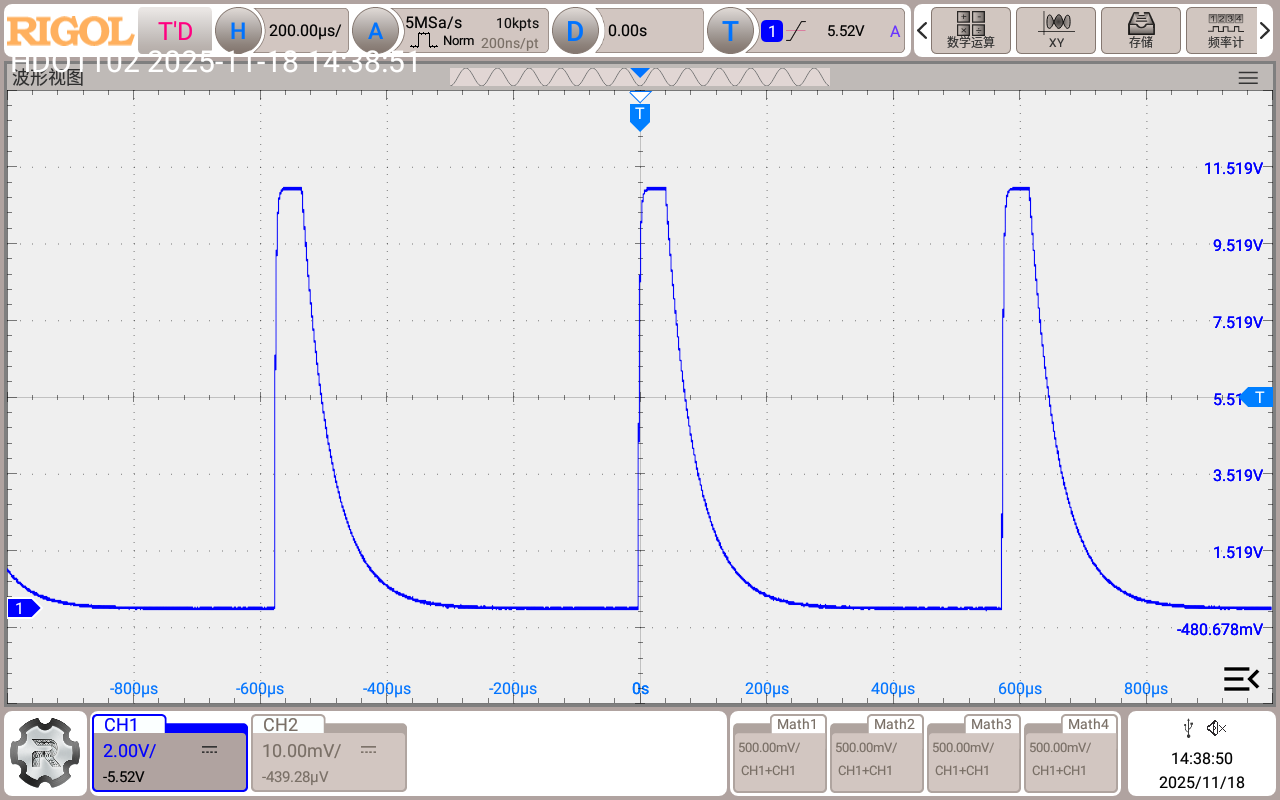
\includegraphics[width=0.4\textwidth, height=0.2\textheight]{figure/c4301030.png}
    \caption{$R=4.3k \Omega, C=1 \times 10^4 pF$零状态响应波形图}
    \label{fig:6.5}
\end{figure}
\begin{figure}[H]
    \centering
    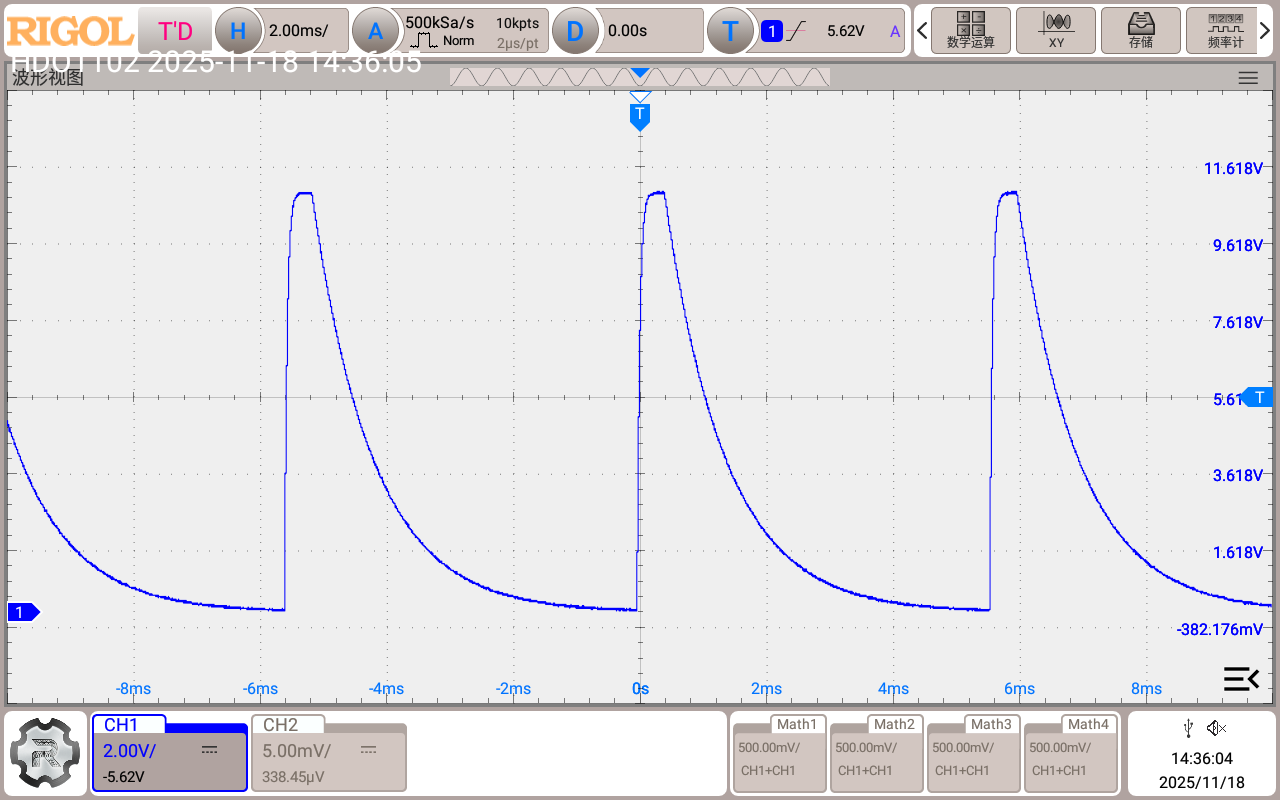
\includegraphics[width=0.4\textwidth, height=0.2\textheight]{figure/c4302240.png}
    \caption{$R=4.3k \Omega, C=2.2 \times 10^5 pF$零状态响应波形图}
    \label{fig:6.6}
\end{figure}

\section*{七、数据分析与讨论}
汇总实验测量结果与计算结果对比如下表所示：
\begin{table}[H]
\footnotesize
\caption{\normalsize  RC电路时间常数计算值与测量值对比} 
\centering  
\renewcommand{\arraystretch}{1.1}
\begin{tabular}{*{5}{l}} 
\hline\hline   
$R(\Omega)$ &$C(pF)$ &$\tau$ 测量值(ms) &$\tau$ 计算值(ms)&相对误差 \\ 
\hline
9.1K & $1 \times 10^{5}$& 0.980& 0.910&7.7\%\\
750 & $1 \times 10^{5}$& 0.086& 0.075&14.7\%\\
4.3K & $1 \times 10^4$& 0.050& 0.043&16.3\%\\
4.3K & $2.2 \times 10^5$& 1.06& 0.946&12.1\%\\
\hline  
    \end{tabular}
    \label{table:7.1}
\end{table}
可以看到实验误差较大。可能原因在于：

1.电阻和电容值由于老化而变动，经过多年实验标称值和实际值有一些偏差，导致时间常数理论值有较大偏差

2.时间常数测量误差。测量时间常数需要在示波器上利用光标法读取坐标，光标难以完全对准，存在偏差。
\section*{八、结论}

通过实验测量了四种不同参数RC电路的时间常数，测量值与理论计算值基本吻合，相对误差在可接受范围内。
实验结果表明，时间常数$\tau=RC$确实决定了电路响应的快慢，电阻或电容值越大，瞬态过程持续时间越长。
实验存在的误差主要来源于元件参数偏差和测量读数误差，但整体上验证了一阶RC电路的瞬态响应特性。
\section*{九、心得与体会}
我通过本实验了解了示波器的使用方法，学会了利用示波器稳定波形，使用自动测量法和光标法测量波形的周期、幅值等

实际观察了RC电路的零输入响应和零状态响应，掌握了测量RC电路时间常数的方法，对RC电路的理解加深。
\section*{十、思考题}
1．什么是零输入响应、零状态响应？ 

零输入响应是指电路在无外部激励信号输入，仅由初始储能（如电容初始电压）作用下的响应过程。零状态响应是指电路初始状态为零（电容初始电压为零），仅由外部激励信号作用下的响应过程。


2．在用示波器观察RC电路响应时如何才能使示波器的扫描与电路激励同步？ 

要使示波器的扫描与电路激励同步，需要将激励信号的前沿作为示波器的外部触发信号。通过调节示波器的触发电平，使触发点稳定在激励信号的特定位置，从而获得稳定的显示波形。

3．什么是时间常数？它在电路中起什么作用？ 

时间常数$\tau=RC$是表征RC电路瞬态响应速度的重要参数。它决定了电容充电或放电的快慢，时间常数越大，充放电过程越缓慢；时间常数越小，充放电过程越迅速。理论上，经过$5\tau$时间后，电路基本达到稳定状态。
\end{document}